\documentclass[12pt]{article}
%\documentclass[10pt, landscape, twocolumn]{article}

\usepackage{setspace}
\onehalfspacing
\usepackage[T2A]{fontenc}
\usepackage[utf8]{inputenc}
\usepackage{amsmath}

\usepackage[lastpage,user]{zref}

\usepackage{geometry, graphics, graphicx}

\graphicspath{ {./images/} }

\geometry
{
    a4paper,
    total={210mm,297mm},
    left=20mm,
    right=20mm,
    top=25mm,
    bottom=20mm,
}

\usepackage{hyperref}

\hypersetup{
    colorlinks=false,       % false: boxed links; true: colored links
    linkcolor=red,          % color of internal links (change box color with linkbordercolor)
    citecolor=green,        % color of links to bibliography
    filecolor=magenta,      % color of file links
    urlcolor=cyan           % color of external links
}

% ------------Колонтитулы-----------------
\usepackage{fancyhdr}
\pagestyle{fancy}

\fancyhead{}
\lhead{\it Задание 1}
\chead{вариант №\,0}
\rhead{\textbf{Выполнили:} ФИО}
\lfoot{\scriptsize\textbf{UPD.:}~\emph{\today}}
\cfoot{}
\rfoot{\thepage /\zpageref{LastPage}}


\usepackage{amsopn}
\DeclareMathOperator{\B}{B}

\usepackage{hyperref}


\usepackage{tikz}
\usepackage{background}
\usepackage{tikzpagenodes}
%\usepackage{lmodern}
\usepackage{indentfirst}

\backgroundsetup%
{   angle=0,
    opacity=2,
    scale=1,
    contents=%
    {   \begin{tikzpicture}[remember picture,scale=3]
            \fontsize{100}{120}\selectfont
            \node[text=gray!50,rotate=90, above=1cm] 	at (current page text area.west) {\textbf{ФН--1}};
            \node[text=gray!50,rotate=-90, above=1cm] 	at (current page text area.east) {\textbf{ФН--1}};          
        \end{tikzpicture}
    }
}
% ----------------------------------------

\newcommand{\ul}{\underline}

\usepackage{amsopn}
\DeclareMathOperator{\up}{up}
\DeclareMathOperator{\h}{h}
\DeclareMathOperator{\fup}{fup}
%\DeclareMathOperator{\ch}{ch}
\DeclareMathOperator{\g}{g}

\usepackage{xcolor}
\definecolor{amaranth}{rgb}{0.9, 0.17, 0.31}
\definecolor{amethyst}{rgb}{0.6, 0.4, 0.8}
\definecolor{ao}{rgb}{0.0, 0.0, 1.0}


\title{Применение свёрточных нейронных сетей в задаче оптического распознавания текста для фильтрации нежелательных данных}
\author{Разумов Т.Е., Чуриков Д.В., Кравченко О.В.}

\begin {document}
\maketitle

\begin{abstract}
В работе рассматривается задача обнаружения и фильтрации нежелательных данных. Решается задача оптического распознавания текста (ОРТ), на примере фильтрации спам-сообщений, получаемых по электронной почте. В качестве модели классификатора нежелательных писем в электронной почте выбрана полносвязная свёрточная нейронная сеть (FCNN), которая разделяет письма на две категории: "спам" и "не спам". Представлен анализ производительности CPU и эффективности обучения модели для различных Python библиотек. Проведены сравнения результатов обучения при различных методах предобработки изображений, содержащих текст: bag of words, word2vec, fast text embeddings. Проведен численный эксперимент, и рассмотрено влияние на скорость и качество обучения модели в зависимости от модификации функции потерь, функций активации на разных слоях, выбора метода оптимизации и изменения иных гипер-параметров. На основе свёрточной сети построена модель потоковой классификации изображений по критерию наличия нежелательной информации, предназначенной для получения идентификационных данных пользователей (фишинга).


Реализовано приложение на языке C++ для запуска классификаторов изображений, имеющее микро-сервисную архитектуру, выдерживающее более 1 млн. запросов в минуту. Сервисы осуществляют взаимодействие по протоколу GRPC, передавая данные в формате protobuf.\\
\textbf{Ключевые слова:} привет, пока, нигер
\end{abstract}


\subsection*{Введение}
Мы живем во время, когда объемы производимой человечеством
информации больше, чем когда либо и количество этих данных растет с каждым
днем. Однако значительную пользу из этой информации можно извлечь лишь
при правильной обработке и анализе этих данных.

{\bf\color{amaranth} (TODO: допиши меня)}


\section{Постановка задачи}
Пусть задано некоторое множество объектов $ X = X_L \cup X_T $, где $X_L$ - обучающая выборка, $X_T$ - тестовая выборка, $Y$ - множество допустимых ответов. Считаем, что существует некоторая целевая функция $g: X \rightarrow Y$, значения которой известны только на множестве $X_L$. Пусть данные распределены в соответствии с некоторым неизвестным распределением $P(x,y) = P(x) P(y|x)$, при этом задана некоторая функция потерь: 
$$
R(g(x), y) = 
\begin{cases} 
0, & y = g(x) \\
> 0, & y \neq g(x)
\end{cases}
$$

В соответствии с принципом минимизации эмпирического риска нам надо минимизировать функцию потерь, то есть найти такую решающую функцию $g(x)$, которая в среднем будет приводить к наименьшей погрешности. Формально, требуется решить следующую задачу минимизации:
$$
g(x) = \operatorname*{argmin}_{f: X \rightarrow Y} E_{X,Y} R(f(x), y)
$$

Для задачи фильтрации нежелательных данных множество $Y$ состоит из двух элементов $\{0, 1\}$, где $0$ и $1$ желательные и нежелательные данные соответственно. В силу грубости методов дискретных вычислений, на практике обычно используется $Y = R[0, 1]$, а результат работы классификатора $y' = g(x)$ отноcится к нужному классу с заданной пороговой вероятностью $\alpha$, минимизирующей ошибку первого и второго рода.


Исходя из потребностей современного общества, мы имеем ограничение 3 секунды на время проверки одного письма, что наклыдвает дополнительные требования к используемым инструментам и остказоустойчивости всей системы. 

\section{``Решение''}
\subsection*{Предобработка текста}
Поскольку текст имеет сильно неоднородную структуру и при этом одно слово может быть записано множеством разных способов (разный шрифт, кодировка, регистр итд), но при этом иметь тот же смысл, то применяются различные методы предобработки текста или их комбинация.

Первым шагом текст производится парсинг и декодирование текста в заданную кодировку. Затем приведение к нижнему (или верхнему) регистру, удаление лишних пробелов, отступов. Производится замена символов по заданному правилу.

{\bf\color{amaranth} (TODO: может быть как то стоит переформулировать).}
После этого применяются следующие методы:

\subsubsection*{\it\,Stop words}
Текст часто содержит много символов, которые не несут смысловой нагрузки для общего смысла (два пробела, абзацный отступ), а также стоп слова (stop words).
Стоп слова -- это слова на любом языке, которые не добавляют особого смысла предложению. 	Часто к стоп словам относят знаки пунктуации, местоимения и предлоги. Часто спамеры используют их для зашумления текстов с целью скрыть спам контент сообщения. Так как их можно спокойно игнорировать, не жертвуя смыслом предложения, то в задачах классификации часто прибегают к их удалению из исходного сообщения.

\subsubsection*{\it\,Стемминг и лемматизация}
Обычно тексты содержат разные грамматические формы одного и того же слова, а также могут встречаться однокоренные слова. Используя разные алгоритмы лемматизация и стемминг преследуют цель привести все встречающиеся словоформы к одной, нормальной словарной форме.


Стемминг -- это грубый эвристический процесс, который отрезает "лишнее" от корня слов, часто это приводит к потере словообразовательных суффиксов. Основная проблема, возникающая при использовании стеммера -- это обработка слов, которые при образовании разных грамматических форм меняют не только окончание, но и основу слова. Например, существительное "кошка" в винительном и родительном падеже множественного числа имеет форму "кошек". Из-за таких беглых гласных стеммер должен либо игнорировать подобные формы, усекая "кошки" до "кошк" и теряя часть форм слова, либо усекать слово до безусловно неизменяющейся основы, получая "кош", что впоследствии может привести к полной потере контекста. Чтобы минимизировать негативные последствия слишком агрессивного усечения слов стеммером, необходимо выполнять стемминг искомого ключевого слова, а затем сравнивать результат с выходом стеммера для каждого из слов в обрабатываемом тексте. Но даже в этом случае буду встречаться совпадения стемов для совершенно несвязанных слов.


Лемматизация -- это более тонкий процесс, который использует словарь и морфологический анализ, чтобы в итоге привести слово к его канонической форме (лемме). Однако он применяет упрощенный анализ слов, не учитывая контекст. Это приводит к неоднозначностям при определении части речи. Например, лемматизация слов в словосочетании "мы роем яму" даст для второго слова два варианта лемматизации: существительное рой и глагол рыть. Эта неоднозначность не может быть разрешена без привлечения морфологического анализатора.

Как правило лемматизация дает наиболее точные результаты и именно этот подход используется в работе.

\subsection*{Векторизация текста}
Современные алгоримы машинного обучения не могут напрямую работать с сырым текстом, поэтому необходимо построить отображение текста в векторное пространство. Это называется извлечением признаков. Рассмотрим несколько подходов для построения данного отображения.

\subsubsection*{\it\,Мешок слов}
Модель "мешок слов" - это упрощенное представления текстовой информации, используемое в задачах обработки естественных языков и поиска информации. В этой модели текст представляется в виде мешка (мультимножества) его слов или словосочетаний в случае комбинаций термов, игнорируя грамматику и в некоторых случаях даже порядок слов, но сохраняя множественность. Каждому такому терму (слову или словосочетанию) ставится в соответствие некоторое число. В этом случае текст определяется вектором $x=(x_1, ..., x_N)^T$, где $N$ - размерность из конечного словаря $X_L$ состоящего из уникальных термов обучающей выборки. Возможны следующие варинаты определения $x_i$:

\begin{itemize}
\item Булевский вес: $\begin{cases} 1, & \mbox{если элемент присутствует в письме} \\ 0, & \mbox{если элемент не присутствует в письме}  \end{cases}$
\item Количество вхождений i-го терма в тексте: $x_i = n_i$
\item Частота терма: $x_i = \dfrac{n_i}{\sum n_k}$
\end{itemize}

В данной работе для определения $x_i$ мы взяли частоту терма.

\subsubsection*{\it\,Word2Vec}

\subsubsection*{\it\,Fast Text}

\subsection*{Классификация текста}
После векторизации текста мы должны построить преобразование из множества признаков во множество классифицируемых объектов $g: X \rightarrow Y$

\subsubsection*{\it\,Логистическая регрессия}
Наиболее частым методом используемым в задаче классификации используется метод логистической регрессии:
$$
g(x) = \dfrac{1}{1 + \exp{ \{ \sum_{i=0}^n w_i x_i  \} }},
$$

где $w=(w_1, ..., w_N)^T$ - веса модели, полученные при обучении.


Задав порог принятия решений равным $\alpha = 0.75$. Приведем результаты расчетов для разных способов векторизации текста.

Для BOW эмбедингов мы имеем следующие результаты:
\begin{center}
  \begin{tabular}{ | c | c | c | c |}
    \hline
      & precision & recall & f1-score \\ \hline
    0 & 0.99896 & 0.79620 & 0.88613 \\ \hline
    1 & 0.91143 & 0.99961 & 0.95348 \\ \hline
    accuracy & \multicolumn{3}{c|}{0.93395} \\                   
    \hline
  \end{tabular}
\end{center}


Для Fast Text эмбедингов мы имеем следующие результаты:
\begin{center}
  \begin{tabular}{ | c | c | c | c |}
    \hline
      & precision & recall & f1-score \\ \hline
    0 & 0.99896 & 0.79620 & 0.88613 \\ \hline
    1 & 0.91143 & 0.99961 & 0.95348 \\ \hline
    accuracy & \multicolumn{3}{c|}{0.93395} \\                   
    \hline
  \end{tabular}
\end{center}
{\bf\color{amaranth} (TODO: внести результаты)}

\subsubsection*{\it\,Fully convolutional neural network}
Для Fast Text эмбедингов мы имеем следующие результаты:
\begin{center}
  \begin{tabular}{ | c | c | c | c |}
    \hline
      & precision & recall & f1-score \\ \hline
    0 & 0.99896 & 0.79620 & 0.88613 \\ \hline
    1 & 0.91143 & 0.99961 & 0.95348 \\ \hline
    accuracy & \multicolumn{3}{c|}{0.93395} \\                   
    \hline
  \end{tabular}
\end{center}
{\bf\color{amaranth} (TODO: внести результаты)}

\subsection*{Реализация алгоритмов}

\subsubsection*{\it\,Обзор библиотек}

\subsubsection*{\it\,Микросервисная архитектура}
\begin{figure}[h!]
	\center
	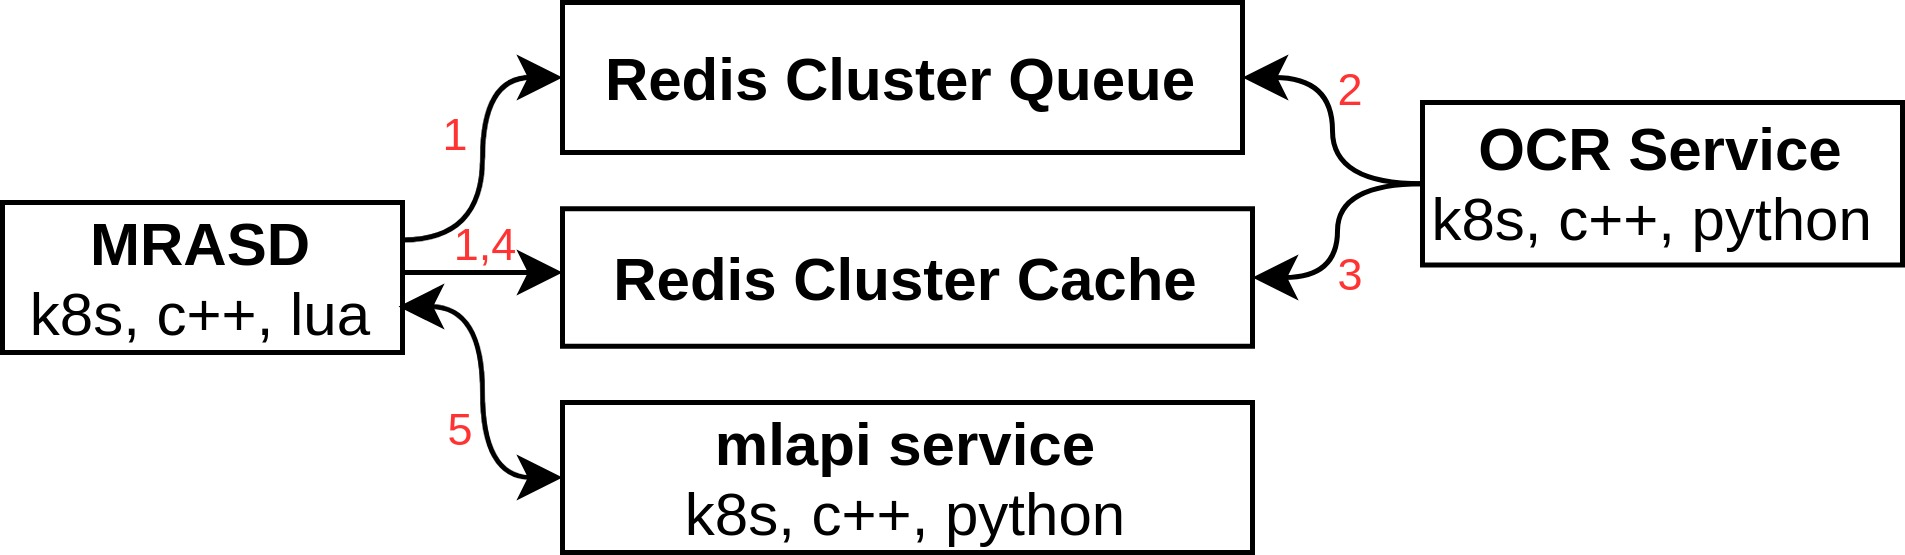
\includegraphics[scale=0.25]{deploy.jpg}
	\caption{График функции $\up(x)$ и $\up'(x)$}
	\label{fig:02}
\end{figure}

\section{Conclusions}

\begin{thebibliography}{99}
\bibitem{Ref01} {\bf\color{ao} Sample \ldots}
\end{thebibliography}

\end {document}
